\chapter{Model Files, Binary Formats, And Runtime Buffers}

An LLM is not only a neural network equation. It is also a collection of files on disk,
arrays in CPU memory, tensors on GPU memory, and temporary buffers created during training
and inference. Many beginner explanations skip this layer, but professional LLM work
depends on it.

This chapter answers a practical question:

\begin{quote}
Are \texttt{*.bin}, \texttt{*.pt}, Candle files, and llm.c files the same thing?
\end{quote}

Short answer:

\begin{quote}
They often store the same \emph{logical objects}, but they organize, serialize, name,
validate, and load those objects differently.
\end{quote}

A token file, a PyTorch checkpoint, a safetensors file, and an llm.c binary checkpoint
may all participate in the same GPT system. They are not interchangeable unless the
project defines a shared contract.

\section{The Four Layers Of An LLM System}

When students say ``the model,'' they may mean four different things:

\begin{enumerate}
  \item \textbf{Model specification}: vocabulary size, context length, layer count,
  hidden dimension, attention heads, activation, normalization, and loss rule.
  \item \textbf{Model parameters}: the learned tensors, such as embedding tables and
  attention projection matrices.
  \item \textbf{Training state}: optimizer moments, scheduler step, gradient scaler,
  random number generator state, and current step.
  \item \textbf{Runtime buffers}: input batches, activations, gradients, attention masks,
  temporary workspaces, and inference KV cache.
\end{enumerate}

These layers should not be confused.

\begin{figure}[htbp]
\centering
\resizebox{\textwidth}{!}{%
\begin{tikzpicture}[
  box/.style={draw, rounded corners, minimum width=3.0cm, minimum height=0.8cm, align=center},
  arrow/.style={-{Latex[length=3mm]}, thick}
]
\node[box, fill=blue!6] (spec) at (0,0) {model spec\\YAML/TOML/JSON};
\node[box, fill=green!10] (params) at (3.6,0) {parameters\\learned tensors};
\node[box, fill=yellow!18] (state) at (7.2,0) {training state\\optimizer, step, RNG};
\node[box, fill=red!8] (buffers) at (10.8,0) {runtime buffers\\activations, KV cache};
\draw[arrow] (spec) -- (params);
\draw[arrow] (params) -- (state);
\draw[arrow] (state) -- (buffers);
\node[align=center, font=\small] at (5.4,-1.25)
{A useful checkpoint explains which of these layers it stores and which must be supplied separately.};
\end{tikzpicture}}
\caption{An LLM system has specification, parameters, training state, and runtime buffers.}
\end{figure}

\section{Token \texttt{.bin}: Data, Not Model Weights}

In this book, \texttt{train.bin} and \texttt{valid.bin} usually mean token data files.
They are not neural network weights. They are arrays of token IDs:

\[
[15496,\ 11,\ 616,\ 1438,\ 318,\ 257,\ldots].
\]

The job of a token \texttt{.bin} file is to let the data loader read token IDs quickly
without repeatedly parsing text.

\subsection{Logical View}

The logical object is:

\[
\text{token stream} \in \mathbb{N}^{N}.
\]

For training, the data loader slices windows:

\[
x = [t_i,t_{i+1},\ldots,t_{i+T-1}],
\qquad
y = [t_{i+1},t_{i+2},\ldots,t_{i+T}].
\]

Then a batch stacks many windows:

\[
X,Y \in \mathbb{N}^{B\times T}.
\]

\begin{figure}[htbp]
\centering
\resizebox{\textwidth}{!}{%
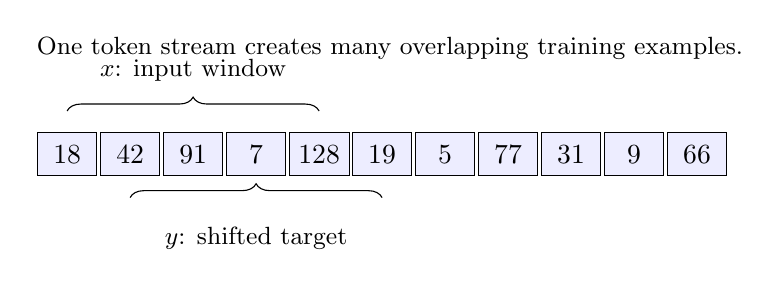
\begin{tikzpicture}[
  tok/.style={draw, minimum width=0.75cm, minimum height=0.55cm, fill=blue!7},
  lab/.style={font=\small, align=center},
  arrow/.style={-{Latex[length=3mm]}, thick}
]
\foreach \i/\v in {0/18,1/42,2/91,3/7,4/128,5/19,6/5,7/77,8/31,9/9,10/66} {
  \node[tok] (t\i) at (\i*0.8,0) {\v};
}
\draw[decorate, decoration={brace, amplitude=5pt}] (0.0,0.55) -- (3.2,0.55)
  node[midway, above=0.25cm, lab] {\(x\): input window};
\draw[decorate, decoration={brace, amplitude=5pt}] (0.8,-0.55) -- (4.0,-0.55)
  node[midway, below=0.25cm, lab] {\(y\): shifted target};
\node[lab] at (4.1,1.35) {One token stream creates many overlapping training examples.};
\end{tikzpicture}}
\caption{A token \texttt{.bin} file stores a one-dimensional stream; the batcher creates \(\shape{[B,T]}\) tensors.}
\end{figure}

\subsection{Physical View}

On disk, the same token stream may be stored as little-endian \texttt{uint16} or
\texttt{uint32}. If the vocabulary has at most 65536 tokens, \texttt{uint16} can be
enough. A 32000-token vocabulary fits in \texttt{uint16}. Larger vocabularies usually need
\texttt{uint32}.

\begin{lstlisting}
data/tokens/wikitext103/
  train.bin
  train.meta.json
  valid.bin
  valid.meta.json
\end{lstlisting}

A serious metadata file should include:

\begin{lstlisting}
{
  "dtype": "uint16",
  "byte_order": "little",
  "num_tokens": 123456789,
  "vocab_size": 32000,
  "tokenizer": "tokenizers/gpt21-bpe-32k.json",
  "tokenizer_sha256": "...",
  "source_dataset": "wikitext103",
  "split": "train"
}
\end{lstlisting}

\term{Important}: the extension \texttt{.bin} is generic. A project may also use
\texttt{.bin} for weights or checkpoints. Always ask: ``What schema does this binary file
obey?''

\section{PyTorch \texttt{.pt}: Flexible Checkpoint Containers}

PyTorch commonly saves checkpoints with extensions such as \texttt{.pt} or \texttt{.pth}.
PyTorch documentation recommends saving a model's \texttt{state\_dict}, which maps tensor
names to tensor values \cite{pytorchsavingloading}.

A training checkpoint may look like:

\begin{lstlisting}[language=Python]
torch.save({
    "model": model.state_dict(),
    "optimizer": optimizer.state_dict(),
    "scheduler": scheduler.state_dict(),
    "step": step,
    "config": config_dict,
    "tokenizer_sha256": tokenizer_hash,
    "rng_state": torch.get_rng_state(),
}, "step-9500.pt")
\end{lstlisting}

The logical object is a dictionary. Some values are tensors. Some are Python scalars or
metadata.

\subsection{What A \texttt{.pt} File Can Contain}

\begin{longtable}{p{0.25\textwidth}p{0.46\textwidth}p{0.16\textwidth}}
\toprule
\term{Object} & \term{Purpose} & \term{Needed for} \\
\midrule
Model weights & learned parameters such as embeddings, attention weights, MLP weights & inference, resume \\
Optimizer state & AdamW moments \(m\) and \(v\) & faithful resume \\
Scheduler state & learning-rate schedule position & faithful resume \\
Step number & where training stopped & resume, logs \\
Config & architecture and training settings & interpretation \\
Tokenizer metadata & vocabulary identity and hash & correct embedding meaning \\
RNG state & random continuation state & reproducibility \\
AMP scaler & mixed precision scale state & stable resume \\
\bottomrule
\end{longtable}

\subsection{Why \texttt{latest.pt} And \texttt{step-9500.pt} Differ}

In the GPT21 run, \texttt{latest.pt} is a moving recovery pointer. A numbered file such as
\texttt{step-9500.pt} is a milestone artifact. They may contain almost the same fields,
but they have different roles:

\begin{itemize}
  \item \texttt{latest.pt}: convenient for crash recovery;
  \item \texttt{step-9500.pt}: stable record for comparison, evaluation, and release;
  \item \texttt{best.pt}: should point to the best validation checkpoint, not necessarily
  the final checkpoint.
\end{itemize}

Professional training keeps all three concepts separate.

\section{Candle And Safetensors: Tensor Archives With Rust Discipline}

Candle is a Rust ML framework. In the Hugging Face ecosystem, \texttt{safetensors} is a
common tensor serialization format designed to store tensors with metadata without
executing arbitrary code during loading \cite{huggingfacesafetensors}. Candle can use this
style naturally because it treats model loading as explicit Rust code.

A Candle-oriented artifact layout can look like:

\begin{lstlisting}
checkpoints/candle-gpt21/
  model.safetensors
  optimizer.safetensors
  config.toml
  tokenizer.json
  training_state.json
  metrics.jsonl
\end{lstlisting}

The distinction is useful:

\begin{itemize}
  \item tensor bytes live in \texttt{*.safetensors};
  \item architecture meaning lives in \texttt{config.toml};
  \item tokenizer meaning lives in \texttt{tokenizer.json};
  \item current training step and schedule position live in \texttt{training\_state.json}.
\end{itemize}

This is less magical than a large Python checkpoint dictionary. That is a strength.
Rust/Candle forces the project to say exactly what exists and how it is loaded.

\section{llm.c Binary Files: Flat Buffers And Explicit Layout}

llm.c-style systems use C/CUDA and therefore prefer simple, explicit memory layouts.
Instead of a Python dictionary mapping names to tensors, a C program often uses:

\begin{itemize}
  \item a small binary header;
  \item a config block;
  \item one large parameter buffer;
  \item views into that buffer for each tensor;
  \item activation and gradient buffers allocated separately at runtime.
\end{itemize}

Conceptually, the same GPT weights exist:

\[
W_{\text{token}}, W_q, W_k, W_v, W_o, W_{\text{mlp}}, W_{\text{vocab}}.
\]

Physically, they may be packed into one long array:

\[
\theta =
[W_{\text{token}}\ |\ W_q\ |\ W_k\ |\ W_v\ |\ W_o\ |\ \cdots ].
\]

\begin{figure}[htbp]
\centering
\resizebox{\textwidth}{!}{%
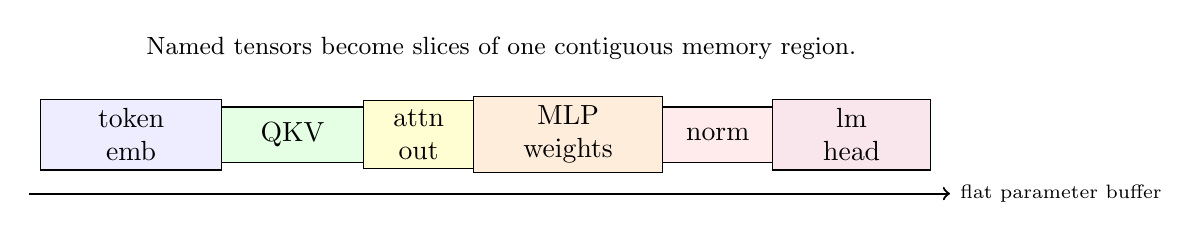
\begin{tikzpicture}[
  seg/.style={draw, minimum height=0.7cm, align=center},
  lab/.style={font=\small, align=center}
]
\node[seg, fill=blue!7, minimum width=2.3cm] at (0,0) {token\\emb};
\node[seg, fill=green!10, minimum width=1.8cm] at (2.05,0) {QKV};
\node[seg, fill=yellow!18, minimum width=1.4cm] at (3.65,0) {attn\\out};
\node[seg, fill=orange!14, minimum width=2.4cm] at (5.55,0) {MLP\\weights};
\node[seg, fill=red!8, minimum width=1.4cm] at (7.45,0) {norm};
\node[seg, fill=purple!10, minimum width=2.0cm] at (9.15,0) {lm\\head};
\draw[->, thick] (-1.3,-0.75) -- (10.4,-0.75) node[right] {\scriptsize flat parameter buffer};
\node[lab] at (4.7,1.1) {Named tensors become slices of one contiguous memory region.};
\end{tikzpicture}}
\caption{A C/CUDA backend may store parameters as named views into a flat buffer.}
\end{figure}

This is not a different model. It is a different memory discipline. The advantage is
performance visibility. The disadvantage is that metadata and shape contracts must be
handled carefully by the project.

\section{Same Logical Tensors, Different Organization}

\begin{longtable}{p{0.18\textwidth}p{0.22\textwidth}p{0.25\textwidth}p{0.22\textwidth}}
\toprule
\term{Layer} & \term{PyTorch} & \term{Candle/safetensors} & \term{llm.c/CUDA} \\
\midrule
Token data &
\texttt{train.bin} read into tensors, often via NumPy or memory map &
same binary token stream, read by Rust code &
same token stream, often optimized for contiguous reads \\
Model config &
Python/YAML dict &
typed Rust config, TOML/JSON/YAML &
C struct or binary header \\
Weights &
\texttt{state\_dict} tensor map in \texttt{.pt} &
tensor archive such as \texttt{model.safetensors} &
flat parameter buffer with named offsets \\
Optimizer &
Python optimizer state dict &
typed optimizer state, possibly tensor archive plus JSON &
manual arrays for moments and updates \\
Activations &
autograd saves tensors automatically &
framework-managed tensors with Rust ownership &
explicit activation buffers and workspaces \\
Inference cache &
PyTorch tensors, easy to inspect &
Rust-owned tensors, product-friendly API &
manual KV cache layout for speed \\
\bottomrule
\end{longtable}

The model is the same if all of these agree:

\begin{enumerate}
  \item same tokenizer;
  \item same token IDs;
  \item same config;
  \item same parameter names or a correct name mapping;
  \item same tensor shapes;
  \item same dtype interpretation;
  \item same forward-pass math;
  \item same decoding rule during inference.
\end{enumerate}

\section{Runtime Buffers During Training}

During training, files are loaded into memory and expanded into several buffer classes.
This is where memory usage grows beyond checkpoint size.

\begin{figure}[htbp]
\centering
\resizebox{\textwidth}{!}{%
\begin{tikzpicture}[
  box/.style={draw, rounded corners, minimum width=2.55cm, minimum height=0.75cm, align=center},
  arrow/.style={-{Latex[length=3mm]}, thick}
]
\node[box, fill=blue!6] (disk) at (0,0) {disk\\\texttt{train.bin}};
\node[box, fill=yellow!16] (cpu) at (3.0,0) {CPU batch\\\(\shape{[B,T]}\)};
\node[box, fill=orange!12] (gpu) at (6.0,0) {GPU tensors\\input, target};
\node[box, fill=green!10] (act) at (9.0,0.9) {activations\\for backward};
\node[box, fill=red!8] (grad) at (9.0,-0.9) {gradients\\and optimizer};
\node[box, fill=purple!10] (params) at (6.0,-1.8) {parameters\\\(\theta\)};
\draw[arrow] (disk) -- (cpu);
\draw[arrow] (cpu) -- (gpu);
\draw[arrow] (gpu) -- (act);
\draw[arrow] (act) -- (grad);
\draw[arrow] (params) -- (gpu);
\draw[arrow] (grad) -- (params);
\end{tikzpicture}}
\caption{Training loads token files, creates batches, runs forward activations, then stores gradients and optimizer state.}
\end{figure}

For AdamW training, memory roughly includes:

\[
\text{parameters} + \text{gradients} + m + v + \text{activations} + \text{temporary buffers}.
\]

This is why a 265 MiB checkpoint may require much more GPU memory during training.

\section{Runtime Buffers During Inference}

Inference does not need optimizer state or backward activations. It does need:

\begin{itemize}
  \item model parameters;
  \item prompt token IDs;
  \item hidden states for the current forward pass;
  \item logits for the next-token distribution;
  \item optionally, a KV cache.
\end{itemize}

The KV cache stores keys and values from previous positions:

\[
K,V \in \mathbb{R}^{L \times B \times H \times T_{\max} \times D_h}.
\]

The cache is not normally part of the checkpoint. It is created at runtime for a specific
prompt or serving request.

\section{How Formats Are Created And Maintained}

\subsection{Creating Token \texttt{.bin}}

\begin{enumerate}
  \item collect raw text;
  \item normalize and clean text;
  \item train or choose tokenizer;
  \item encode text into token IDs;
  \item choose dtype, usually \texttt{uint16} or \texttt{uint32};
  \item write contiguous binary IDs;
  \item write metadata JSON with tokenizer hash and token count.
\end{enumerate}

\subsection{Creating PyTorch \texttt{.pt}}

\begin{enumerate}
  \item instantiate model from config;
  \item train for some steps;
  \item collect model \texttt{state\_dict};
  \item collect optimizer, scheduler, scaler, step, and metadata;
  \item call \texttt{torch.save};
  \item verify load on a clean process.
\end{enumerate}

\subsection{Creating Candle Artifacts}

\begin{enumerate}
  \item instantiate the typed Rust model from config;
  \item save tensor weights into a tensor archive;
  \item save non-tensor metadata in JSON/TOML;
  \item verify tokenizer/config/checkpoint hashes;
  \item run a deterministic forward-pass test after reload.
\end{enumerate}

\subsection{Creating llm.c-Style Artifacts}

\begin{enumerate}
  \item define a binary header and version;
  \item write model dimensions;
  \item write parameters in a fixed order;
  \item document each tensor's shape and offset;
  \item write conversion scripts from PyTorch or safetensors if needed;
  \item validate with a tiny deterministic forward pass.
\end{enumerate}

\section{GGUF: A Single-File Inference Format}

GGUF, short for GGML Universal File, is a binary file format used by GGML-based inference
engines such as \texttt{llama.cpp}. The official specification describes it as a format
for storing models for inference with GGML executors, designed for fast loading, saving,
\texttt{mmap} compatibility, extensibility, and enough embedded information to load the
model without separate user-supplied hyperparameters \cite{ggufspec}.

This makes GGUF different from a training checkpoint. A GGUF file is usually an
\emph{export artifact}. The model may be trained in PyTorch, Candle, or llm.c, then
converted into GGUF for local inference.

\begin{figure}[htbp]
\centering
\resizebox{\textwidth}{!}{%
\begin{tikzpicture}[
  box/.style={draw, rounded corners, minimum width=2.7cm, minimum height=0.75cm, align=center},
  arrow/.style={-{Latex[length=3mm]}, thick}
]
\node[box, fill=blue!6] (train) at (0,0) {training\\checkpoint};
\node[box, fill=yellow!18] (convert) at (3.4,0) {conversion\\script};
\node[box, fill=green!10] (gguf) at (6.8,0) {GGUF\\inference file};
\node[box, fill=red!8] (runtime) at (10.2,0) {llama.cpp\\Ollama-style runtime};
\draw[arrow] (train) -- (convert);
\draw[arrow] (convert) -- (gguf);
\draw[arrow] (gguf) -- (runtime);
\node[align=center, font=\small] at (5.1,-1.1)
{GGUF is normally downstream from training, not the primary training resume file.};
\end{tikzpicture}}
\caption{A common production path converts a training checkpoint into a GGUF inference artifact.}
\end{figure}

\subsection{What Is Inside A GGUF File?}

At a high level, a GGUF file contains:

\begin{lstlisting}
GGUF file
  header
    magic bytes
    version
    tensor count
    metadata count

  metadata key-value table
    architecture name
    context length
    embedding length
    layer count
    head count
    tokenizer information
    quantization information
    rope settings
    special token IDs

  tensor information table
    tensor name
    tensor dimensions
    tensor type
    byte offset into tensor data block

  tensor data block
    aligned binary tensor bytes
    often FP16, BF16, Q8, Q6, Q5, Q4, etc.
\end{lstlisting}

The important design idea is \term{self-description}. A GGUF reader can inspect metadata,
know how many tensors exist, locate each tensor by offset, and load the weights into a
GGML runtime.

\subsection{GGUF Is Not A Full Training Checkpoint}

GGUF is excellent for inference deployment, but it usually should not be treated as the
canonical training checkpoint. It normally does not contain:

\begin{itemize}
  \item AdamW optimizer moment tensors;
  \item learning-rate scheduler state;
  \item gradient scaler state;
  \item random number generator state;
  \item training dataloader position;
  \item full experiment logs.
\end{itemize}

That is why the \texttt{llm-train} pipeline should keep both:

\begin{itemize}
  \item a faithful training checkpoint for resume and research;
  \item a GGUF export for local inference and product testing.
\end{itemize}

\subsection{GGUF And Quantization}

GGUF is often associated with quantized models. Quantization stores weights with fewer
bits than FP16 or FP32. For example, a model may be exported as Q8, Q6, Q5, or Q4. This
reduces disk size and memory use, often making local CPU or small-GPU inference possible.

Quantization changes the physical representation of the weights:

\[
\text{FP16 weights} \rightarrow \text{quantized blocks + scale information}.
\]

The logical tensor is still a weight matrix, but its bytes are no longer a simple dense
FP16 array. This is one reason GGUF is an inference format: the runtime knows how to
multiply with those quantized blocks efficiently.

\subsection{Where GGUF Fits In The Three-Backend Story}

\begin{longtable}{p{0.20\textwidth}p{0.32\textwidth}p{0.32\textwidth}}
\toprule
\term{Source backend} & \term{Native training artifact} & \term{GGUF role} \\
\midrule
PyTorch & \texttt{.pt}, \texttt{.pth}, or \texttt{safetensors} plus config/tokenizer & export after validation for llama.cpp/Ollama-style inference \\
Candle & \texttt{model.safetensors}, Rust config, tokenizer, training state & export if the model architecture and tensor names can be mapped to GGUF conventions \\
llm.c & custom \texttt{.bin} checkpoints and token/data artifacts & either export to Hugging Face format first or write a direct GGUF exporter \\
\bottomrule
\end{longtable}

The export step must prove correctness. After conversion, compare:

\begin{enumerate}
  \item tokenizer identity;
  \item model dimensions;
  \item tensor name mapping;
  \item greedy next-token output on fixed prompts;
  \item validation or perplexity on a small held-out set if the runtime supports it;
  \item sample metadata and decoding settings.
\end{enumerate}

\section{Converting Trained Models To GGUF}

The most common GGUF conversion path today expects a Hugging Face-style model directory.
llama.cpp provides \texttt{convert\_hf\_to\_gguf.py}, a Python script that reads model
configuration, tokenizer files, tensor names, and tensor data, then writes a GGUF file
\cite{llamacppconvertgguf}. Therefore, the clean training-pack strategy is:

\[
\text{backend checkpoint}
\rightarrow
\text{canonical HF-style export}
\rightarrow
\text{GGUF}
\rightarrow
\text{optional quantized GGUF}.
\]

\begin{figure}[htbp]
\centering
\resizebox{\textwidth}{!}{%
\begin{tikzpicture}[
  box/.style={draw, rounded corners, minimum width=2.7cm, minimum height=0.75cm, align=center},
  arrow/.style={-{Latex[length=3mm]}, thick}
]
\node[box, fill=blue!6] (torch) at (0,1.2) {PyTorch\\\texttt{.pt}};
\node[box, fill=green!10] (candle) at (0,0) {Candle\\safetensors};
\node[box, fill=orange!12] (llmc) at (0,-1.2) {llm.c\\custom \texttt{.bin}};
\node[box, fill=yellow!18] (hf) at (4.0,0) {canonical export\\HF-style folder};
\node[box, fill=purple!10] (gguf) at (7.8,0) {FP16/BF16\\GGUF};
\node[box, fill=red!8] (quant) at (11.2,0) {quantized\\GGUF};
\draw[arrow] (torch) -- (hf);
\draw[arrow] (candle) -- (hf);
\draw[arrow] (llmc) -- (hf);
\draw[arrow] (hf) -- (gguf);
\draw[arrow] (gguf) -- (quant);
\end{tikzpicture}}
\caption{A robust GGUF pipeline converts backend-specific checkpoints through a canonical model export.}
\end{figure}

\subsection{Step 1: Select The Source Checkpoint}

Do not convert a random checkpoint merely because it exists. Select a checkpoint using
evidence:

\begin{itemize}
  \item validation loss and perplexity;
  \item sample quality on fixed prompts;
  \item tokenizer/config hash match;
  \item no known training corruption;
  \item clear license and dataset notes.
\end{itemize}

For the GPT21 WikiText-103 run, the best listed validation point was step 8250. A release
pipeline should evaluate \texttt{step-8250.pt}, \texttt{step-9500.pt}, and
\texttt{step-9999.pt}, then choose the checkpoint intentionally.

\subsection{Step 2: Export To A Canonical Directory}

A conversion script needs more than raw tensors. It needs architecture metadata and
tokenizer metadata. A practical intermediate directory is:

\begin{lstlisting}
exports/gpt21-hf/
  config.json
  tokenizer.json
  tokenizer_config.json
  special_tokens_map.json
  model.safetensors
  generation_config.json        optional
  README.md                     model card / export notes
\end{lstlisting}

The \texttt{config.json} must describe the architecture in names the converter
understands. This is the hardest part for a new architecture. If the converter does not
know \texttt{GPT21ForCausalLM}, either:

\begin{itemize}
  \item export using a compatible architecture class if the model is truly compatible;
  \item add a model mapping to the conversion code;
  \item write a project-owned GGUF exporter using the GGUF Python writer;
  \item postpone GGUF export until the architecture contract is stable.
\end{itemize}

\subsection{Step 3: Convert HF-Style Export To GGUF}

The common llama.cpp command shape is:

\begin{lstlisting}
python3 /path/to/llama.cpp/convert_hf_to_gguf.py \
  exports/gpt21-hf \
  --outfile exports/gpt21-f16.gguf \
  --outtype f16
\end{lstlisting}

The exact supported \texttt{--outtype} values can change with llama.cpp, so always check:

\begin{lstlisting}
python3 /path/to/llama.cpp/convert_hf_to_gguf.py --help
\end{lstlisting}

The conversion should emit a log that shows:

\begin{itemize}
  \item detected architecture;
  \item tokenizer handling;
  \item tensor names read from source;
  \item GGUF tensor names written;
  \item output dtype;
  \item output file path.
\end{itemize}

\subsection{Step 4: Quantize The GGUF File}

Many GGUF deployments use quantization. A common workflow is to first write a full or
half-precision GGUF, then quantize it with a llama.cpp quantization tool:

\begin{lstlisting}
/path/to/llama.cpp/build/bin/llama-quantize \
  exports/gpt21-f16.gguf \
  exports/gpt21-q4_k_m.gguf \
  Q4_K_M
\end{lstlisting}

Binary names and paths differ by platform and build system, so the book focuses on the
artifact flow rather than one permanent path:

\[
\text{source checkpoint}
\rightarrow
\text{FP16 GGUF}
\rightarrow
\text{Q8/Q6/Q5/Q4 GGUF}.
\]

\subsection{Step 5: Verify The Export}

A GGUF export is not complete until it has passed checks:

\begin{longtable}{p{0.25\textwidth}p{0.55\textwidth}}
\toprule
\term{Check} & \term{What to verify} \\
\midrule
Metadata & architecture, context length, embedding size, layers, heads, tokenizer fields \\
Tensor inventory & every expected tensor exists with expected shape \\
Tokenizer & same prompt becomes same token IDs where possible \\
Greedy prompt & deterministic short generation resembles the source model \\
Quantization drift & quantized output remains acceptable for the deployment target \\
Runtime & file loads in llama.cpp/Ollama-style runtime without hidden assumptions \\
Manifest & export command, source hash, output hash, quantization type, and tester are recorded \\
\bottomrule
\end{longtable}

\subsection{PyTorch, Candle, And llm.c Conversion Notes}

\begin{longtable}{p{0.18\textwidth}p{0.30\textwidth}p{0.34\textwidth}}
\toprule
\term{Source} & \term{Best conversion path} & \term{Main risk} \\
\midrule
PyTorch \texttt{.pt} &
load \texttt{state\_dict}, export \texttt{model.safetensors} plus HF-style config/tokenizer &
checkpoint may contain training-only names or missing tokenizer metadata \\
Candle &
save named tensors as safetensors and write a compatible config/tokenizer directory &
Rust model tensor names may need mapping to converter names \\
llm.c &
read custom binary checkpoint, unpack flat buffers, write canonical named tensors &
offset/order mistakes can silently corrupt weights \\
\bottomrule
\end{longtable}

The safest conversion policy is to make tensor-name mapping explicit and test it with a
tiny deterministic model before converting a large trained checkpoint.

\section{Industry Model Format Landscape}

The LLM ecosystem uses several file conventions:

\begin{longtable}{p{0.17\textwidth}p{0.24\textwidth}p{0.40\textwidth}}
\toprule
\term{Format} & \term{Common role} & \term{Notes} \\
\midrule
\texttt{.pt}/\texttt{.pth} & PyTorch checkpoint & flexible, convenient for training, often contains Python metadata and optimizer state \\
\texttt{.safetensors} & tensor archive & common for model weights, safer loading model than pickle-style Python objects, needs config/tokenizer beside it \\
\texttt{*.bin} token files & training data shards & raw token ID arrays; not the same as model weights \\
\path{pytorch_model.bin} & older Hugging Face weight file naming & name contains \texttt{.bin}, but it is model weights, not token data \\
custom C binary & systems backend checkpoint & fast and explicit, but project-specific \\
\texttt{.gguf} & GGML/llama.cpp inference model & self-contained metadata plus tensors, often quantized, good for local inference but not a full training resume checkpoint \\
other quantized inference formats & deployment & store reduced-precision weights for inference, often not suitable for continued training \\
\bottomrule
\end{longtable}

The extension is less important than the schema. A file is professional when it can answer:

\begin{itemize}
  \item What tensors or arrays are inside?
  \item What are their names, shapes, dtypes, and byte order?
  \item What config gives those tensors meaning?
  \item What tokenizer gives embedding rows meaning?
  \item What backend wrote the file?
  \item What version of the schema is this?
  \item How do we verify that loading preserved behavior?
\end{itemize}

\engineering

For \texttt{llm-train}, define a shared artifact contract:

\begin{lstlisting}
artifacts/
  token_shard:
    path: data/tokens/wikitext103/train.bin
    dtype: uint16
    endian: little
    tokenizer_sha256: ...
  model_config:
    vocab_size: 32000
    block_size: 512
    n_layer: 6
    n_head: 6
    n_embd: 384
  checkpoint:
    backend: torch_reference | candle_rust | llmc_cuda
    format: pt | safetensors | llmc_binary | gguf
    step: 9500
    config_sha256: ...
    tokenizer_sha256: ...
    role: train_resume | eval_candidate | inference_export
\end{lstlisting}

Then each backend may store bytes differently while still proving that it implements the
same model.

\section{Hands-On Lab: Inspect A Token \texttt{.bin}}

Write or use a script that prints:

\begin{itemize}
  \item file size;
  \item dtype;
  \item number of tokens;
  \item first 32 token IDs;
  \item decoded first 32 tokens;
  \item tokenizer hash.
\end{itemize}

Explain why the file cannot be interpreted without dtype and tokenizer metadata.

\section{Hands-On Lab: Inspect A PyTorch \texttt{.pt}}

Load a checkpoint on CPU and print only metadata and tensor shapes:

\begin{lstlisting}[language=Python]
ckpt = torch.load("step-9500.pt", map_location="cpu")
print(ckpt.keys())
for name, tensor in ckpt["model"].items():
    print(name, tuple(tensor.shape), tensor.dtype)
\end{lstlisting}

Then answer:

\begin{itemize}
  \item Which tensors are parameters?
  \item Is optimizer state present?
  \item Is tokenizer metadata present?
  \item Could this checkpoint be used for inference only?
  \item Could this checkpoint faithfully resume training?
\end{itemize}

\section{Hands-On Lab: Design A Cross-Backend Manifest}

Create a file called \texttt{artifact\_manifest.json}. It should describe one token shard,
one PyTorch checkpoint, one Candle checkpoint, and one llm.c checkpoint. Include:

\begin{itemize}
  \item paths;
  \item backend;
  \item schema version;
  \item tensor or token dtype;
  \item config hash;
  \item tokenizer hash;
  \item validation loss if known;
  \item command used to create the artifact.
\end{itemize}

\checkpoint

\begin{enumerate}
  \item Why is \texttt{train.bin} not a model checkpoint?
  \item Why can two files with extension \texttt{.bin} mean totally different things?
  \item What does a PyTorch \texttt{state\_dict} map?
  \item Why is tokenizer metadata required to interpret embedding weights?
  \item What is the difference between parameters and runtime buffers?
  \item Why does training need more memory than inference?
  \item Why does a Candle/safetensors-style layout often separate tensors from metadata?
  \item What is the advantage of llm.c-style flat buffers?
  \item What should be tested after converting a checkpoint between formats?
  \item Why should \texttt{latest.pt} not be treated automatically as the best model?
\end{enumerate}

\subsection*{Solutions}

\begin{enumerate}
  \item \texttt{train.bin} stores token IDs, which are data examples. A checkpoint stores
  model parameters and possibly training state.
  \item File extensions are conventions, not schemas. One project may use \texttt{.bin}
  for token IDs; another may use it for model weights.
  \item A \texttt{state\_dict} maps parameter or buffer names to tensor values.
  \item Embedding row \(i\) only has meaning if token ID \(i\) has the same tokenizer
  meaning used during training.
  \item Parameters are learned persistent tensors. Runtime buffers are temporary memory
  used for batches, activations, gradients, workspaces, or KV cache.
  \item Training stores activations for backward pass, gradients, and optimizer moments.
  Inference usually needs only parameters, current activations, logits, and possibly KV
  cache.
  \item It makes loading explicit and portable: tensors are stored as tensors, while
  architecture and tokenizer meaning are stored in structured metadata.
  \item Flat buffers reduce indirection and make memory layout visible, which helps C/CUDA
  performance engineering.
  \item Compare config, tokenizer hash, tensor names, shapes, dtypes, a deterministic
  forward pass, loss, and greedy next-token output.
  \item \texttt{latest.pt} is usually the most recent recovery checkpoint. The best model
  should be selected by validation loss and sample evaluation.
\end{enumerate}
